\documentclass[a4paper,twoside]{article}
\usepackage{autiwa}

\title{Aide mémoire emacs}
\author{Christophe \textsc{Cossou}}

\newcommand{\raccourci}[1]{{\bfseries #1}}

\makeindex
\begin{document}

\tableofcontents

\clearpage
\section{Informations de base}
Ce tutoriel n'est qu'un résumé condensé des commandes d'emacs. Je l'ai rédigé au fur et à mesure de la lecture et l'apprentissage du tutoriel emacs disponible \emph{dans} \gras{emacs}.
\subsection{Comment faire les raccourcis}
\og \raccourci{C}\fg correspond à la touche \touche{Ctrl}

\og \raccourci{M}\fg correspond à la touche \touche{Meta}, c'est à dire la touche \touche{cmd} sous mac (et sans doute la touche \touche{Alt} sous windows et GNU/Linux)

\og \raccourci{<RET>}\fg correspond à un appui sur la touche \touche{Entrée} du clavier.

\begin{remarque}
Le raccourci \raccourci{C-g} permet d'annuler toute saisie de commande en cours (et donc en particulier des raccourcis).
\end{remarque}

\begin{exemple}
Quand dans la suite du document je dirais de faire le raccourci \raccourci{C-p}, il s'agira de faire \touche{Ctrl}+\touche{p}, pour faire \raccourci{M-f}, il faut faire \touche{cmd}+\touche{f} sous mac (ou \touche{Alt}+\touche{f} sous windows et GNU/Linux)
\end{exemple}

\begin{remarque}
Faire précéder la plupart des raccourcis de \raccourci{C-u \emph{n}}, où $n$ est un nombre entier de répétition que l'on souhaite permet de réitérer la commande. 

Un exemple simple et parfois utile est de répéter un caractère : 
\begin{exemple}
\raccourci{C-u 10 *} permet de répéter 10 fois une astérisque
\end{exemple}

\end{remarque}


\section{Pour se déplacer dans le document}
Pour se déplacer d'une ligne à l'autre il faut faire \raccourci{C-p} (\emph{previous}) ou \raccourci{C-n} (\emph{next}).

Pour se déplacer d'un caractère il faut faire \raccourci{C-b} (\emph{backward}) ou \raccourci{C-f} (\emph{forward}).

Pour se déplacer d'un mot, il faut faire \raccourci{M-b} (\emph{backward}) ou \raccourci{M-f} (\emph{forward}).

Pour aller au début ou à la fin de la ligne il faut faire \raccourci{C-a} (début) ou \raccourci{C-e} (\emph{end})

Pour aller au début ou à la fin de la phrase (paragraphe en pratique) il faut faire \raccourci{M-a} (début) ou \raccourci{M-e} (\emph{end})

Pour se déplacer d'une page (il recopie les deux dernières lignes) il faut faire \raccourci{C-v} pour descendre d'une page ou \raccourci{M-v} pour remonter d'une page.

\bigskip

\raccourci{C-l} place la ligne courante au milieu de la page puis au début puis en bas (et par cycle) ; ceci avant de faciliter la lecture.

\raccourci{M-g} permet de spécifier le n° de ligne auquel on veut aller. 

\begin{remarque}
Dans la pratique, pour pouvoir me servir de ce raccourci afin d'aller à la ligne 112 par exemple, je dois faire : 

\raccourci{M-g} + \raccourci{M-g} et enfin spécifier '112' quand il affiche 'Goto line:' et enfin appuyer sur \touche{Entrée}.
\end{remarque}


\section{Effacer du texte}\index{texte!effacer}
Pour supprimer le reste de la ligne : \raccourci{C-k}

Pour supprimer un mot : \raccourci{M-d} supprime le mot sous le curseur tandis que \raccourci{M-Del} supprime le mot à gauche du curseur.

\bigskip

On peut aussi décider de supprimer une zone de caractères et non une succession de lignes comme l'illustre \reffig{fig:array_selection}.

Pour poser une marque, il suffit de faire \raccourci{C-Space} (ou \raccourci{C-@}). Puis placez le curseur à la fin de la zone que vous souhaitez effacer ou déplacer (la zone sera sélectionnée comme illustré sur \reffig{fig:array_selection}). Pour ensuite couper la zone, faites \raccourci{C-x r k}. 

\begin{remarque}
Ce dernier type de commande est une commande qui s'applique sur un \emph{rectangle}. D'où la signification du 'r' dans le raccourci. On \emph{exécute} (\raccourci{C-x}) sur un \emph{rectangle} (\raccourci{r}) une commande particulière, ici \raccourci{k} pour \emph{kill}. Pour plus de détails, se référer à \refsec{sec:rectangles}.
\end{remarque}


\section{Couper/Copier/coller du texte}\index{texte!couper}\index{texte!copier}\index{texte!coller}
Afin de copier du texte, il faut le sélectionner puis faire \raccourci{Esc-w}. Pour le coller, il suffit de faire \raccourci{C-y}.

\begin{remarque}
Pour Copier, la commande standard est normalement \raccourci{M-w} mais sous mac ça ne fonctionne pas. À la place il veut me quitter le buffer en cours\dots
\end{remarque}

Afin de couper du texte, il faut le sélectionner puis faire \raccourci{C-w}. Pour le coller, il suffit de faire \raccourci{C-y}.

\bigskip

Pour couper du texte, toutes les autres commandes d'effacement fonctionnent. 

\begin{remarque}\index{kill-ring}
Pour copier/coller du texte, on dispose d'un mécanisme puissant : le \emph{kill-ring}. À chaque fois qu'une portion de texte est copiée (ou collée) elle est placée dans une liste. Pour coller, on utilise \raccourci{C-y}, suivi directement de \raccourci{M-y} si on veut accéder aux autres éléments du \emph{kill-ring}.
\end{remarque}

\bigskip

On peut aussi décider de supprimer une zone de caractères et non une succession de lignes comme l'illustre \reffig{fig:array_selection}.

\begin{figure}[htb]
\centering
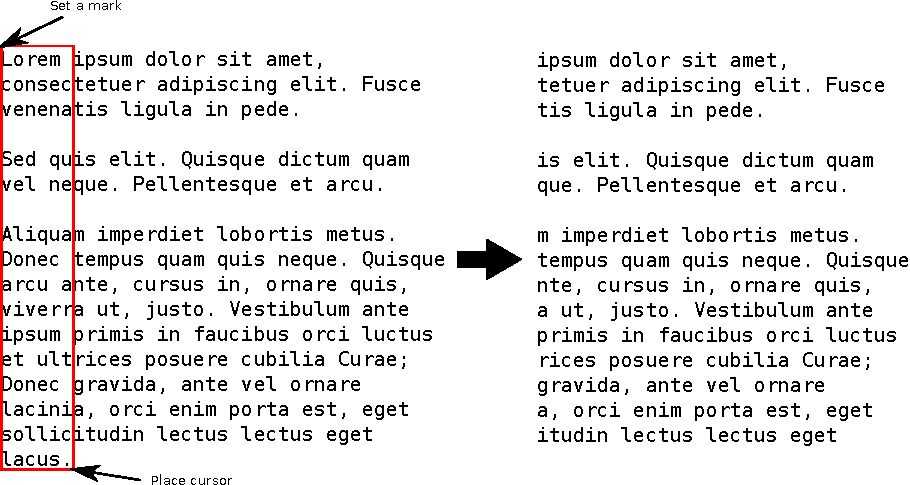
\includegraphics[width=0.7\linewidth]{../vectoriel/emacs_array_selection.pdf}
\caption{On souhaite supprimer la zone encadrée. Il faut pour celà mettre le marqueur dans le coin en haut à gauche et placer le curseur en bas à droite. Ensuite faire \raccourci{C-x r k}.}\label{fig:array_selection}
\end{figure}

Pour poser une marque, il suffit de faire \raccourci{C-Space} (ou \raccourci{C-@}). Puis placez le curseur à la fin de la zone que vous souhaitez effacer ou déplacer (la zone sera sélectionnée comme illustré sur \reffig{fig:array_selection}). Pour ensuite couper la zone, faites \raccourci{C-x r k}. 

Si vous souhaitez ensuite insérer cette zone quelque part, il faut faire \raccourci{C-x r y}.


\section{Raccourcis utiles}
\begin{important}
\raccourci{C-g} permet d'arrêter une commande en cours ou de supprimer un début de raccourci que vous auriez commencé à écrire.
\end{important}


\raccourci{C-x u} permet d'annuler la dernière commande

\raccourci{C-x C-f} permet d'ouvrir un nouveau fichier

\raccourci{C-x C-s} permet de sauvegarder le fichier courant

\raccourci{C-x C-b} permet d'afficher la liste des fichiers ouverts (buffers)

\raccourci{C-x b} permet de passer à un autre fichier (comme des onglets en quelque sorte)

\raccourci{C-x 1} permet de fermer tous les autres fichiers ouverts et de ne garder que le fichier courant

\section{Rechercher du texte}
\raccourci{C-s} (\emph{search}) ouvre une invite de commande où on peut taper ce que l'on cherche. Cette recherche est incrémentale, c'est à dire qu'il va chercher à mesure que vous écrivez ce que vous cherchez (il va chercher 'c', puis 'cu', puis 'cur' jusqu'à 'curseur').

\raccourci{C-s} permet de rechercher l'occurence suivante, \raccourci{<Delback>} pour rechercher en arrière.

Il suffit de faire \raccourci{Entrée} pour mettre fin à la recherche.

\bigskip

Pour aller à la ligne n°$n$ il suffit de faire \raccourci{C-g g}, d'entrer le nombre voulu (ici $n$) puis de valider avec \touche{Entrée}.

\section{Auto-indentation}
Découvert par hasard, le raccourci \raccourci{Shift+Tab} permet d'indenter correctement tout un bout de code. 

\begin{exemple}
Si vous sélectionnez le code suivant :
\begin{verbatim}
for i=0,nsets-1 do begin

for k=0,nr-1 do begin
for j=0,nt-1 do begin
sigma2(j,k)=data(k,j,i)
endfor
sigmean(k)=mean(sigma2(*,k))
endfor

if (i EQ 0) then begin
plot,r,sigmean,_EXTRA=e
endif else begin
oplot,r,sigmean,col=255*i/nsets
endelse

endfor
\end{verbatim}
et que vous entrez le raccourci \raccourci{Shift+Tab}, vous obtiendrez\footnotemark alors :
\begin{verbatim}
for i=0,nsets-1 do begin

   for k=0,nr-1 do begin
      for j=0,nt-1 do begin
         sigma2(j,k)=data(k,j,i)
      endfor
      sigmean(k)=mean(sigma2(*,k))
   endfor

   if (i EQ 0) then begin
      plot,r,sigmean,_EXTRA=e
   endif else begin
      oplot,r,sigmean,col=255*i/nsets
   endelse

endfor
\end{verbatim}

\end{exemple}
\footnotetext{À condition d'être dans un mode définissant un language de programmation (et donc une indentation particulière). En effet, en mode \emph{fundamental}, l'indentation résultante n'avait pas de sens, ceci parce que les mots clés pour les boucles doivent être définis.}


\section{Changer la casse}
\subsection{D'un mot}
Pour mettre en majuscule : \raccourci{M-u} (\emph{uppercase})

Pour mettre en minuscule : \raccourci{M-l} (\emph{lowercase})

Pour mettre en majuscule uniquement la première lettre du mot : \raccourci{M-c} (\emph{capitalize})

\begin{remarque}
Pour que ceci s'applique sur le texte sélectionné, il faut faire \raccourci{C-x C-u} et \raccourci{C-x C-l} en lieu et place de \raccourci{M-u} et \raccourci{M-l}. Si aucun texte n'est sélectionné, il s'applique au mot courant.
\end{remarque}

\section{Pour aller plus loin}
\subsection{Opérations sur les rectangles}\label{sec:rectangles}
Pour une illustration de ce qu'est un rectangle, se référer à \reffig{fig:array_selection}.

Si le point et la marque sont dans la même colonne, le rectangle qu'ils délimitent sera vide. S'ils sont dans la même ligne, le rectangle aura une seule ligne. Cette asymétrie entre les lignes et les colonnes vient du fait que le point (et la marque de la même manière) sont situées entre deux colonnes, mais sur une ligne.

\bigskip

\raccourci{C-x r k} permet de couper le texte contenu dans le rectangle, le sauvant en tant que dernier rectangle coupé (avec possibilité de le coller ensuite).

\raccourci{C-x r d} supprime le texte contenu dans le rectangle sans possibilité de le coller ensuite. Ceci permet de ne pas effacer le dernier rectangle coupé (vu qu'il n'y a pas de \emph{kill-ring} pour les rectangles mais une seule occurence gardée en mémoire.

\raccourci{C-x r y} colle le dernier rectangle couper avec le coin en haut à gauche du rectangle placé là où se trouve le curseur (point).

\raccourci{C-x r o} insère des espaces pour remplir le rectangle sélectionné. Ceci déplace le texte contenu dans le rectangle vers les colonnes de droite.

\raccourci{C-x r t string <RET>} remplace le contenu de chaque ligne du rectangle sélectionné par \texttt{string}.

\raccourci{M-x string-insert-rectangle <RET> string <RET>} insère \texttt{string} sur chaque ligne du rectangle, déplaçant le texte précédemment contenu dans ce dernier sur les colonnes à droite.


\end{document}